% Breve descripción de la técnica que utilizará para resolver el problema, descripción del algoritmo base a utilizar.

\subsection{Origen biológico}

El principio de selección clonal es un modelo que explica la forma en la cual el sistema inmune
responde a una determinada infección y como algunos tipos de linfocitos T y B son seleccionados
para destruir un determinado antígeno que está invadiendo el cuerpo del sujeto.

Fue propuesto por el virólogo australiano, Sir Frank Macfarlane Burnet en el año 1959,
con un trabajo titulado \emph{``The clonal selection theory of acquired immunity''}.

Existen cuatro postulados fundamentales en la hipótesis de la selección clonal, los cuales son detallados más adelante:
\begin{enumerate}
	\item Cada linfocito soporta un solo tipo de receptor con una única especificación.
	\item La ocupación del receptor es requerida para la activación de la célula.
	\item Las células efectoras diferenciadas derivadas desde un linfocito activado soportarán receptores de una especificación idéntica al de la célula padre.
	\item Aquellos linfocitos que soportan receptores para moléculas propias serán eliminados en una etapa temprana.
\end{enumerate}

De acuerdo a la teoría propuesta por Burnet, el repertorio del sistema inmune se somete a un mecanismo de selección durante el tiempo de vida de un individuo.
La teoría establece que al unirse con un antígeno adecuado, se produce la activación de los linfocitos.
Una vez activado, los clones de los linfocitos son producidos con receptores idénticos a los linfocitos originales que encontraron el antígeno.
Así ocurre una expansión clonal de los linfocitos originales.
Esto asegura que solo los linfocitos específicos que se han activado gracias a un antígeno sean producidos en grandes cantidades.
La teoría de la selección clonal también establece que cualquier linfocito que tenga receptores de antígenos de moléculas propias del organismo
debe ser eliminada durante el desarrollo de los linfocitos.
Esto asegura que solo los antígenos de un patógeno pueden causar que un linfocito se clone y se expanda y así generar una respuesta inmune adaptativa a
agentes externos.
Durante la expansión clonal de linfocitos B, el promedio de la afinidad entre los anticuerpos aumenta para el antígeno que desencadena la expansión clonal.
Este fenómeno se llama maduración de la afinidad, y es responsable de el hecho de que en una posterior exposición al antígeno, la respuesta inmune es más eficaz debido a los anticuerpos con una mayor afinidad por el antígeno.
La maduración de la afinidad es causada por una hiper-mutación somática y un mecanismo de selección que ocurre durante la expansión clonal de linfocitos B.
La hiper-mutación somática altera la especificación de los anticuerpos, introduciendo cambios aleatorios a los genes que lo forman.
\begin{figure}[h!]
\begin{center}
\includegraphics[width=0.3\textwidth]{img/clonalSelection.pdf}
\end{center}
\caption{Ejemplo de una selección clonal de linfocitos}
\label{fig:clonalSelection}
\end{figure}

Se señala la descripción de la figura~\ref{fig:clonalSelection} se detalla a continuación:
\emph{(1)} Una célula madre hematopoyética se somete a la diferenciación y
la reordenación genética para producir \emph{(2)} linfocitos inmaduros con
varios receptores de antígenos distintos.
Aquellos que se unen a \emph{(3)} antígenos de los tejidos del propio cuerpo
son destruidas, mientras que el resto madura y se convierten en \emph{(4)} linfocitos
inactivos. La mayoría de ellos nunca encontrarán un patógeno correspondiente \emph{(5)}
antígeno exterior, pero aquellas que se activan y producen (6) muchos clones de sí mismos.

\subsection{Algoritmo de la Selección Clonal}



Siguiendo el principio de selección clonal y el proceso de maduración de la afinidad, postulado por De Castro~\cite{decastro} se puede describir el algoritmo de selección clonal de la siguiente forma:
\begin{figure}[h!]
\begin{center}
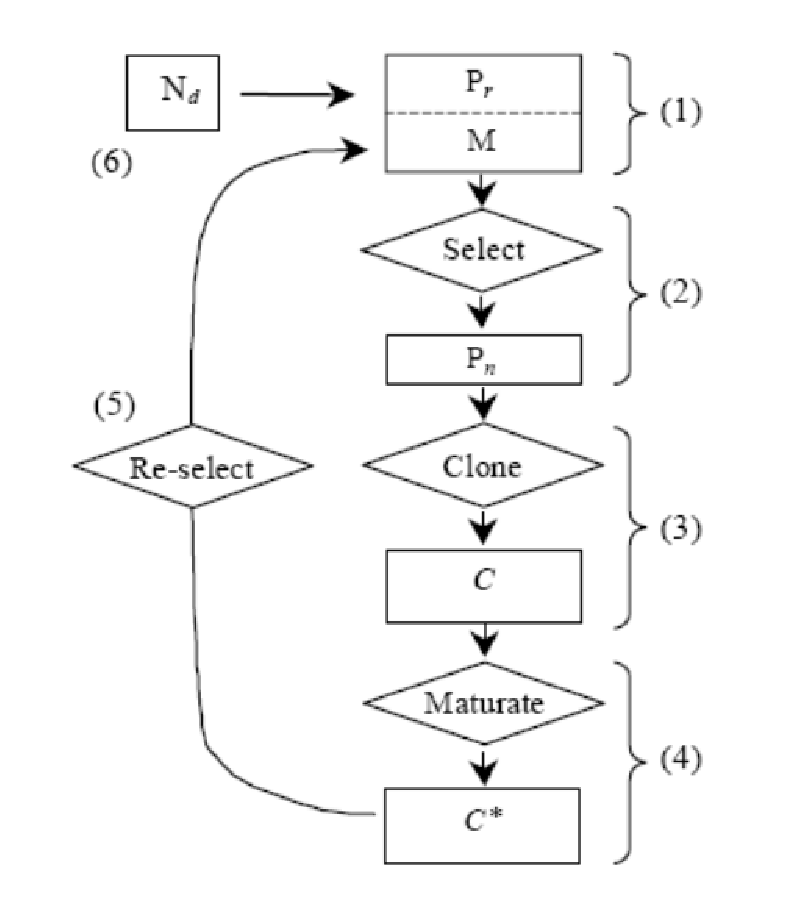
\includegraphics[width=0.5\textwidth]{img/algoritmo}
\end{center}
\caption{Diagrama del algoritmo de la selección clonal}
\label{fig:algoritmo}
\end{figure}

Siendo la explicación de los pasos de la figura~\ref{fig:algoritmo} la siguiente:
\begin{enumerate}
    \item Generar un conjunto (P) de soluciones candidatas, compuesto de células de memoria (M) añadidas a la población restante (Pr), teniendo entonces $P = Pr + M$
    \item Determinar los $n$ mejores individuos (Pn) de la población (P), basado en una medida de afinidad.
    \item Clonar (reproducir) estos $n$ mejores individuos de la población, dando origen a una población temporal de clones (C).
    \item Someter la población de clones a un esquema de hiper-mutación (proporcional a la afinidad del anticuerpo). Una población de anticuerpos maduros es generada (C*).
    \item Seleccionar nuevamente los mejores individuos de (C*) para componer el conjunto de memoria. (Algunos reemplazos desde (C*) a (P), debido a la mejora)
    \item Reemplazar los $d$ anticuerpos con menor afinidad de la población, manteniendo la diversidad.
\end{enumerate}

